\newcommand{\anonsection}[1]{\section*{#1}\addcontentsline{toc}{section}{#1}}
\newcommand{\anonsubsection}[1]{\subsection*{#1}\addcontentsline{toc}{subsection}{#1}}
\newcommand{\anonsubsubsection}[1]{\subsubsection*{#1}\addcontentsline{toc}{subsubsection}{#1}}

\documentclass[11pt]{article}

\usepackage[T2A]{fontenc}
\usepackage[utf8]{inputenc}
\usepackage[russian]{babel}

\usepackage{indentfirst}
\usepackage{geometry}
\usepackage{graphicx}
\usepackage{caption}
\usepackage{subcaption}
\usepackage{mathtools}

\usepackage{amsmath, amssymb, amsfonts, amsthm}

\newtheorem{theorem}{Теорема}
\newtheorem{definition}{Определение} 
\newtheorem{statement}{Утверждение}
\newtheorem{property}{Свойство}

\DeclareMathOperator{\Uni}{\mathbb{U}}
\DeclareMathOperator{\Ind}{\mathbb{I}}
\DeclareMathOperator{\Bin}{\mathrm{Bin}}
\DeclareMathOperator{\Bern}{\mathrm{Bern}}
\DeclareMathOperator{\Geom}{\mathrm{Geom}}
\DeclareMathOperator{\Norm}{\mathrm{N}}
\DeclareMathOperator{\Expon}{\mathrm{Exp}}
\DeclareMathOperator{\Pois}{\mathrm{Pois}}
\DeclareMathOperator{\Exp}{\mathbb{E}}

\geometry{a4paper}
\sloppy

\begin{document}

\begin{titlepage}
    \begin{centering}
        
\includegraphics[width=0.5\textwidth]{resources/msu.png}\\
        {\scshape Московский государственный университет имени М.~В.~Ломоносова}\\
        Факультет вычислительной математики и кибернетики\\
        Кафедра системного анализа\\
        \vfill
        {\LARGE Отчет по компьютерному практикуму к курсу}\\
        \vspace{1cm}
        {\Huge\bfseries "<Стохастический анализ и моделирование">\\}
    \end{centering}
    \vspace{1cm}
    \begin{flushright}
        \begin{large}
            {\itshape Студент 415 группы\\}
            Е.~В.~Гуров\\
            \vspace{5mm}
            {\itshape Руководитель практикума\\}
            к.ф.-м.н., доцент С.~Н.~Смирнов\\
        \end{large}
    \end{flushright}
    \vfill
    \begin{centering}
        Москва, 2022\\ 
    \end{centering}
\end{titlepage}

\newpage
\setcounter{page}{2}
\tableofcontents
\newpage

\anonsection{Задание 1}

\anonsubsection{Формулировка задания}

\begin{enumerate}
	\item Реализовать генератор схемы Бернулли с заданной вероятностью
     успеха $p$. На основе генератора схемы Бернулли построить датчик
     для биномиального распределения.
	\item Реализовать генератор геометрического распределения. Проверить
     для данного распределения свойство отсутствия памяти.
	\item Рассмотреть игру в орлянку - бесконечную последеовательность
     независимых испытаний с бросанием правильной монеты.
     Выигрыш $S_n$ определяется как сумма по всем $n$ испытаниями 1 и -1
     в зависимости от выпавшей стороны. Проиллюстрировать (в виде ломанной)
     поведение нормированной суммы $Y(i) = S_i / \sqrt{n},$ как функцию
     от номера испытания $i = 1, \dots, n$ для одной отдельно взятой
     траектории. Дать теоритическую оценку для $Y(n)$
     при $n \longrightarrow \infty$.
\end{enumerate}

\anonsubsection{Генератор схемы Бернулли и биномиального распределения}
\begin{definition}
	Схемой Бернулли называется эксперимент, в котором проводится,
     вообще говоря, неограниченное количество испытаний. При этом каждому
     испытанию присваивается бинарный признак (успех --- $1$ или неудача --- $0$), и
     выполняются следующие требования:
	\begin{enumerate}
		\item отсутствие взаимного влияния;
		\item воспроизводимость;
		\item испытания проводятся в сходных условиях.
	\end{enumerate}
\end{definition}

\begin{definition}
	Случайная величина $X$, принимающая значение $1$ с вероятностью
     $p$ и значение $0$ с вероятностью $q = 1 - p$, называется случайной величиной
     с распределением Бернулли(или бернуллиевской случайной величиной).
\end{definition}

Для генератора схемы Бернулли реализуем генератор бернуллиевской случайной
 величины $X$. Для этого воспользуемся встроенным в библиотеку Numpy
 языка Python генератором равномерного распределения. Пусть тогда имеем
 случайную величину $Y \sim \Uni([0,1])$. В таком случае $X$
 можно представить в виде: $X = \Ind(Y < p)$, где $\Ind()$
 --- индикаторная функция:
$$
    X = \Ind(Y < p) = 
    \begin{cases}
        1 \ , & Y < p, \\
        0 \ , & Y \ge p.
    \end{cases}
$$
Генерация схемы Бернулли в таком случае будет происходить с помощью некоторого
 количества генераций бернуллиевской случайной величины.

\begin{definition}
	Случайная величина $X$ имеет биномиальное распределение с параметрами
     $n$ и $p$ $(X \sim \Bin(n,p))$, если
	$$ \mathbb{P}(X = k) = C^k_n p^k (1 - p)^{n - k}, \quad k \in
     \mathbb{N} \cup \{0\}. $$
\end{definition}

Случайную величину $X$ обычно интерпретируют как число успехов в схеме
 из $n$ испытаний Бернулли с вероятностью успеха $p$ в каждом. Поэтому
$$ X = \sum_{i = 1}^n Y_i ,$$
 где $Y_i \sim \Bern(p) \ , \ i = 1,\dots,n.$

 Промоделируем биномиальное распределение с параметрами $n = 50$, $p = 0.3$
 с помощью генерации схемы Бернулли с $n$ испытаниями:
 
 \begin{figure}[h]
	\begin{center}
		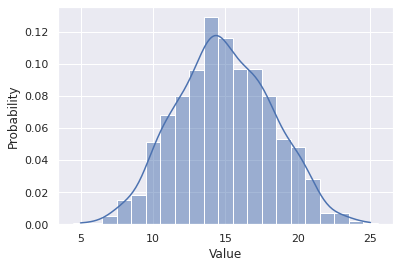
\includegraphics[width=0.85\linewidth]{"./resources/binominal.png"}
		\caption{Гистограмма биномиального распределения с $p = 0.3$, $n = 50$.}
          \label{fig:bin_dist}
	\end{center}
\end{figure}

\anonsubsection{Геометрическое распределение}

\begin{definition}
	Случайная величина $X$ имеет геометрическое распределение с
      параметром $p$ $(X\sim \Geom(p))$, если
	$$ \mathbb{P}(X = k) = (1 - p)^kp = q^k p \ , \ k \in \mathbb{N} \cup 
     \{0\}. $$
\end{definition}

Так же, как и в случае биномиального распределения, проводится некоторое
 количество испытаний Бернулли с одинаковой вероятностью успеха, до
 первого успеха. В качестве случайной величины с геометрическим распределением
 берется, как правило, количество неудач до первого успеха.

\anonsubsection{Свойство отсутствия памяти}
Случайная величина с геометрическим распределением обладает так называемым
 свойством отсутствия памяти. Неформально оно означает, что в момент проведения
 очередного испытания Бернулли количество прошлых неудач не влияет на количество
 будущих. Формально же это свойство можно сформулировать как
\newtheorem{stat}{Утверждение}
\begin{statement}
	Пусть $Y \sim \Geom(p)$, тогда $\forall m,n \in \mathbb{N} \cup 
     \{0\}$ справедливо:
	$$ 
     \mathbb{P}(Y > m + n \mid Y \ge m) = \mathbb{P}(Y > n),
     $$
\end{statement}
\begin{proof} Рассмотрим левую часть равенства:
     \begin{multline*}
          \mathbb{P}(Y > m + n \mid Y \ge m) = \dfrac{\mathbb{P}
          (Y > m + n, Y \ge m)}{\mathbb{P}(Y \ge m)} = \\
          = \dfrac{\mathbb{P}(Y > m + n)}{\mathbb{P}(Y \ge m)} = 
          \dfrac{\displaystyle\sum_{i = m + n + 1}^\infty q^i p}
          {\displaystyle\sum_{i = m}^\infty q^i p} = \dfrac{q^{m + n + 1}}{q^m} =
          q^{n + 1}.
     \end{multline*}
     С другой стороны, правая часть равна:
     $$ 
     \mathbb{P}(Y > n) = \sum_{i = n + 1}^\infty q^i p = p \dfrac{q^{n + 1}}
     {1 - q} = q^{n + 1}.
     $$
\end{proof}

Для демонстрации этого свойства в Python сгенерируем массив некоторого
 достаточного количества геометрических случаных величин. С помощью него
 построим гистограмму геометрического распределения (Рис. \eqref{subfig:geometric_distribution}). Зафиксируем некоторое $m$,
 и построим гистаграмму распределения вектора геометрических случайных
 величин из первоначального набора, значения которых больше либо равны $m$.
 В результате увидим, что при достаточно большом количестве чисел в первоначальном
 наборе гистограммы двух распределений приблизительно совпадают (Рис. \eqref{subfig:memoryless}). 

 \begin{figure}
     \centering
     \begin{subfigure}[b]{0.45\textwidth}
         \centering
         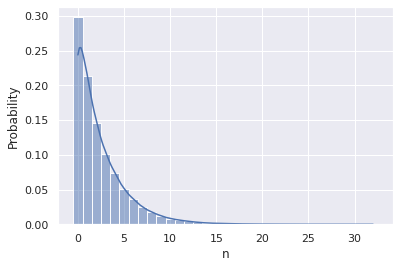
\includegraphics[width=\textwidth]{./resources/geometric.png}
         \caption{Гистограмма геометрического распределения при $p = 0.3$}
         \label{subfig:geometric_distribution}
     \end{subfigure}
     \hfill
     \begin{subfigure}[b]{0.45\textwidth}
         \centering
         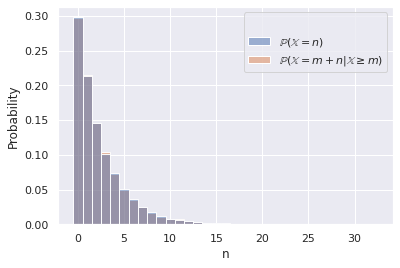
\includegraphics[width=\textwidth]{./resources/comparison.png}
         \caption{Демонстрация свойства отсутствия памяти}
         \label{subfig:memoryless}
     \end{subfigure}
     \caption{}
     \label{fig:geometric}
\end{figure}

\anonsubsection{Игра в орлянку}
Рассмотрим игру в орлянку. Для этого смоделируем последовательность
 случайных величин $X_1, X_2, \dots,$ где
$$
	X_i = 
	\begin{cases}
	     1 \ , & p = \frac{1}{2}\\
	     -1 \ , & p = \frac{1}{2}
	\end{cases}
     ,\quad i = 1,\dots,n.
$$
Тогда необходимая сумма представляется в виде:
$$
Y(i) = \dfrac{X_1 + \dots + X_i}{\sqrt n}, \quad
 i = 1,\dots,n ,
$$
где $n$ --- общее число генераций.

\begin{figure}[h]
	\begin{center}
		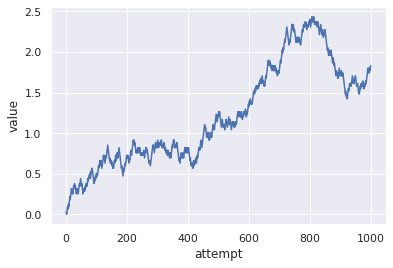
\includegraphics[width=0.75\linewidth]{"./resources/toss_game.png"}
		\caption{Траектория суммы $Y$ с $n = 1000$.}
	\end{center}
\end{figure}

Оценим $Y(n)$ при $n \to \infty$. Для этого сформулируем необходимую
 теорему.
\begin{theorem}[Центральная предельная теорема]
     Пусть $X_1,\dots, X_n,\dots$ есть бесконечная
      последовательность независимых одинаково распределенных случайных
      величин, имеющих конечное математическое ожидание $\mu$ и
      диспрерсию $\sigma^2$. Пусть также
     $$
     S_n = \displaystyle\sum_{i = 1}^n X_i
     $$
     Тогда
     $$
     \dfrac{S_n - \mu n}{\sigma \sqrt{n}} \to \Norm(0,1)
     $$
     по распределению при $n \to \infty$,
     где $\Norm(0,1)$ --- нормальное распределение с нулевым математическим ожиданием
      и стандартным отклонением, равным единице.
\end{theorem}

В случае игры Орлянки:
$$
\mu = \Exp[X_i] = 0, \quad
\sigma^2 = \Exp[(X_i - \Exp[X_i])^2] = 1, \quad i = 1, \dots, n
$$
Тогда поолучим, что последовательность случайных величин
$$
Y_n = Y(n) = \dfrac{S_n}{\sqrt{n}}
$$
Удовлетворяет условиям теоремы 1. Таким образом получаем, что $Y(n) \to \Norm(0,1)$.
\anonsection{Задание 2}
\begin{enumerate}
	\item Построить датчик сингулярного распределения, имеющий в качестве функции
     распределения канторову лесницу. С помощью критерия Колмогорова убедиться в
     корректности работы датчика.
	\item Для канторовых случайных величин проверить свойство симметричности
     относительно $\frac{1}{2}$ ($X$ и $1 - X$ распределены одинаково) и самоподобия
     относительно деления на 3 (условное распределение $Y$ при условии
     $Y \in [0, 1/3]$ совпадает с распределением $\frac{Y}{3}$) с помощью критерия
     Смирнова.
	\item Вычислить значение математическое ожидание и дисперсии для данного
     распределения. Сравнить теоритические значения с эмпирическими для разного объема
     выборок. Проиллюстрировать сходимость.
\end{enumerate}

\anonsubsection{Датчик сингулярного распределения}

\anonsection{Задание 3}
\anonsubsection{Формулировка задания}
\begin{enumerate}
	\item Построить датчик экспоненциального распределения. Проверить для
     данного распределения свойство отсутствия памяти. Пусть $X_1, X_2,
     \dots, X_n$ --- независимо экспоненциально распределенные с. в. с
     параметрами $\lambda_1, \lambda_2, \dots, \lambda_n$ соответственно.
     Найти распределение случайной величины $Y = \min(X_1, X_2, \dots, X_n)$.
	\item На основе датчика экспоненциального распределения построить датчик
     пуассоновского распределения.
	\item Построить датчик пуассоновского распределения как предел
     биномиального распределения. С помощью критерия хи-квадрат Пирсона
     убедиться, что получен датчик распределения Пуассона.
	\item Построить датчик стандартного нормального распределения методом
     моделирования случайных величин парами с переходом в полярные координаты.
     Проверить при помощи t-критерия Стьюдента равенство математических
     ожиданий, а при помощи критерия Фишера равенство дисперсий.  
\end{enumerate}

\anonsubsection{Датчик экспоненциального распределения}
\begin{definition}
	Случайная величина $X$ имеет экспоненциальное распределение с параметром
     $\lambda > 0$, если ее функция распределения имеет вид:
	\begin{equation}\label{exp_func}
	    F_X(x) = 
        \begin{cases}
	        1 - e^{-\lambda x}, &x \geqslant 0,\\
	        0, &x < 0.
	    \end{cases}
	\end{equation}
\end{definition}

\begin{theorem}[Метод обратной функции]\label{theor_inverse}
    Пусть функция распредления $ F $ имеет обратную $ F^{-1} $. Тогда
     функцией распределения случайной величины
    $$
     X = F^{-1}(Y),
    $$
     где $ Y \sim \Uni[0,1]$, является $ F $.
\end{theorem}
\begin{proof}
    Найдем функцию распределения $ X $:
    $$
     F_X(x) = \mathbb{P}(X < x) = \mathbb{P}(F^{-1}(Y) < x) =
      \mathbb{P}(Y < F(x)) = F(x).
    $$
\end{proof}

В случае экспоненциального распределения функция распределения \eqref{exp_func}
 удовлетворяет условиям теоремы и обратная к ней легко выражается:
$$
    F_X^{-1}(y) = -\frac{1}{\lambda} \ln(1 - y).
$$
Суперпозиция $ F(Y) $,где $ Y \sim \Uni[0,1] $ является случайной величиной,
 имеющей экспоненциальное распределение с параметром $ \lambda $:
$$
 X = -\frac{1}{\lambda} \ln(1 - Y) \sim \Expon(\lambda).
$$
На Рис.\eqref{fig:exp_dist} приведено сравнение полученной эмпирически,
 с помощью построенного датчика, плотности экспоненциального распределения
 и его теоретической плотности, представимой в виде:
$$
p(x) = \lambda e^{-\lambda x}
$$
при $ \lambda = 0.5 $.

 \begin{figure}[ht]
	\centering
	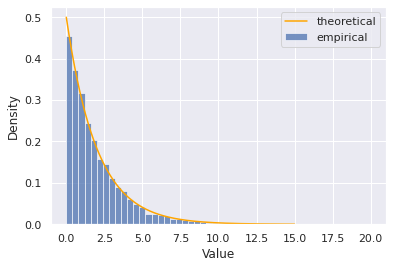
\includegraphics[width = 0.8\linewidth]{"./resources/exp_dist.png"}
	\caption{Эмпирическая и теоретическая плотности экспоненциального
     распределения при $ \lambda = 0.5 $.}
    \label{fig:exp_dist}
\end{figure}

\anonsubsection{Свойство отсутствия памяти}
Экспоненциальное распределение, как и его дискретный аналог --- геометрическое,
 обладает свойством отсутствия мапяти, которое в данном случае можно сформулировать
 как
\begin{statement}
	Случайная величина $X\sim \Expon(\lambda)$ обладает свойством отсутствия памяти,
     то есть $ \forall s,t \ge 0 $ следует, что
	\begin{equation}\label{expmem}
	    \mathbb{P} (X \ge s + t \mid X \ge t) = \mathbb{P} (X \ge s). 
	\end{equation}
\end{statement}
\begin{proof}
	$$
	\mathbb{P}(X \ge s + t \mid X \ge t) = \frac{\mathbb{P}(X \ge s + t, X \ge t}
	 {\mathbb{P}(X \ge t)} = \frac{\mathbb{P} (X \ge s + t)}{\mathbb{P}(t \ge t)}
	 = \mathbb{P}(X \ge s). 
	$$
	Таким образом, получаем:
	\begin{equation}
		\mathbb{P}(X\ge s+t)=\mathbb{P}(X\ge t)\mathbb{P}(X\ge s). \label{equi}
	\end{equation}
	Для экспоненциально распределенной случайной величины верно, что:
	$$
	\mathbb{P} (X \ge t) = 1 - F_X(t) = e^{-\lambda t}, \quad
	\mathbb{P} (X \ge s + t) = e^{-\lambda(s + t)}.
	$$
	Следовательно, для \eqref{equi} выполняется:
	$$
	e^{-\lambda(s + t)} = e^{-\lambda s} e^{-\lambda t}.
	$$
	Следовательно, экспоненциальное распределение обладает свойством отсутствия
	 памяти.
\end{proof}
На Рис.\eqref{fig:exp_memoryless}, аналогично геометрическому распределению,
 данное свойство проиллюстрировано эмпирически.
\begin{figure}[ht]
	\centering
	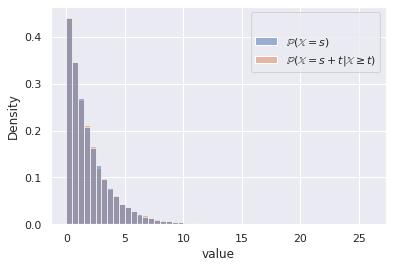
\includegraphics[width = 0.8\linewidth]{"./resources/exp_memoryless.png"}
	\caption{Эмпирическая иллюстрация свойства отсутствия памяти при t = 2.}
    \label{fig:exp_memoryless}
\end{figure}

\anonsubsection{Случайная величина $ Y = \min(X_1, X_2, \dots, X_n) $}
\begin{statement}
	Пусть $ X_1,X_2,\ldots,X_n $ --- независимые экспоненциально распределённые
	 случайные величины с параметрами $ \lambda_1,\lambda_2,\ldots,\lambda_n $
	 соответственно. Тогда случайная величина $ Y = \min(X_1, X_2, \dots, X_n)
	 \sim \Expon \left( \sum\limits_{i = 1}^n \lambda_i \right) $.
\end{statement}
\begin{proof}
	\begin{multline*}
		F_Y(x) = \mathbb{P}(Y \le x) = 1 - \mathbb{P} (Y > x) = 1 - \mathbb{P}
		 (\min(X_1, X_2, \dots, X_n) > x) = \\
		= 1 - \mathbb{P}(X_1 > x, X_2 > x, \dots, X_n > x) = \left\{ X_1, X_2,
		 \dots, X_n \text{ независимы} \right\} = \\
		= 1 - \mathbb{P} (X_1 > x) \cdot \mathbb{P} (X_2 > x) \cdot \dots
		 \mathbb{P} (X_n > x) = \\
		= 1 - \left( 1 - F_{X_1}(x) \right) \cdot \left( 1 - F_{X_2}(x) \right) 
		\cdot \dots \cdot \left( 1 - F_{X_n}(x) \right) = \\
		= 1 - e^{-\lambda_1 x} \cdot e^{-\lambda_2 x} \cdot \dots \cdot
		 e^{-\lambda_n x} = 1 - e^{-\left( \sum_{i=1}^n \lambda_i \right) x}.
	\end{multline*}
\end{proof}
Эмпирическая демонстрация этого факта для n = 4, и случайно сгенерированных
 в интервале от 0 до 0.1 параметров $\lambda_i $ приведена на Рис.\eqref{fig:exp_min}.
\begin{figure}[ht]
	\centering
	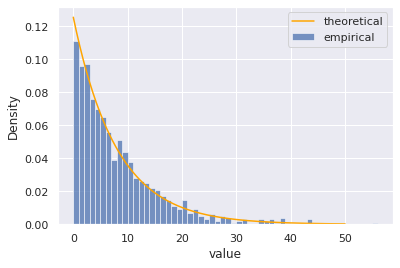
\includegraphics[width = 0.8\linewidth]{"./resources/exp_min.png"}
	\caption{Расределение $ Y = \min(X_1, \dots, X_n) $.}
    \label{fig:exp_min}
\end{figure}

\anonsubsection{Датчик пуассоновского распределения}
\begin{definition}
	Случайная величина $X$ имеет распределение Пуассона с параметром $\lambda>0$,
	 если
	$$
	\mathbb{P}(X = k) = \frac{\lambda^k}{k!} e^{-\lambda}, \quad k \in \mathbb{N} 
	\cup \{0\}.
	$$
\end{definition}
Удобный метод построения датчика пуассоновского распределения даёт следующая 
\begin{theorem}\footnote{Доказательство теоремы можно найти в \cite{model_randoms}
	 на стр. 34.}
	Пусть $X_1,X_2,\ldots,X_n,\ldots\sim Exp(\lambda)$ --- независимые одинаково
	 распредленные случайные величины. Тогда случайная величина, определенная
	 следующим образом:
	$$
	Y = \max(n \mid S_n = X_1 + X_2 + \dots + X_n < 1)
	$$
	имеет распределение Пуассона с параметром $\lambda$. При этом полагается $Y=0$,
	 если таких $ n $ не существует.
\end{theorem}
 Таким образом для моделирования случайной величины Пуассона можно последовательно
 генерировать показательные случайные величины, пока их сумма не станет больше
 единицы. Количество сгенерированных экспоненциальных величин минус один и будет
 значением пуассоновской случайной величины. На Рис.\eqref{fig:pois_dist} изображено
 сравнение распределения выборки полученной с помощью построенного вышеописанным
 способом датчика и теоретической функции вероятности.

\begin{figure}[ht]
	\centering
	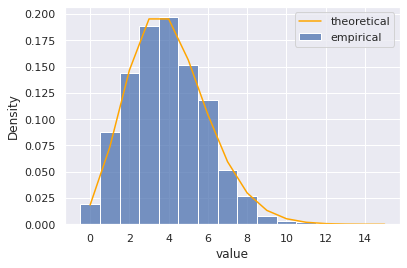
\includegraphics[width = 0.8\linewidth]{"./resources/pois_dist.png"}
	\caption{Эмпирическая и теоретическая плотности распределения Пуассона при
	 $ \lambda = 4 $.}
    \label{fig:pois_dist}
\end{figure}

\anonsubsection{Датчик пуассоновского распределения как предел биномиального 
 распределения}
Другой способ моделирования пуассоновской случайной величины основывается на 
 следующей предельной теореме, связывающей распределение Пуассона с биномиальным
 распределением.
Пусть
$$
P_n(k) = 
\begin{cases}
	C_n^k p^k q^{n-k}, & k = 0, 1, \dots, n,\\
	0, & k = n + 1, n + 2, \dots, 
\end{cases}
$$
и пусть $ p $ является функцией от $ n, \ p = p(n) $.
\begin{theorem}[Пуассона]\footnote{Доказательство этой теоремы можно найти в
	 \cite{shir_prob} на стр. 90.}
	Пусть $ p(n) \to 0, n \to \infty $, причем так, что $ n p(n) \to \lambda $,
	 где $ \lambda > 0 $. Тогда для любого $ k = 0, 1, \dots $
	$$
	P_n(k) \to \dfrac{\lambda^k e^{-k}}{k!}, \quad k = 0, 1, \dots .
	$$
\end{theorem}
Таким образом строить датчик распределения Пуассона с параметром $ \lambda $
 можно с помощью датчика биномиального распределения при $ p =
 \dfrac{\lambda}{n} $ и больших значениях $ n $. На Рис.\eqref{fig:pois_binlim}
 проиллюстрировано достаточно хорошее совпадение распределений $ \Bin\left( n,
 \dfrac{\lambda}{n} \right) $ и $ \Pois(\lambda) $ при $ n = 10000, \lambda = 10 $.

\begin{figure}[ht]
	\centering
	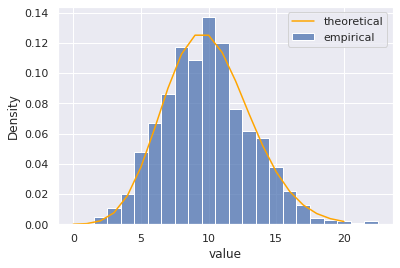
\includegraphics[width = 0.8\linewidth]{"./resources/pois_binlim.png"}
	\caption{Демонстрация предельного совпадения биномиального и пуассоновского
	 распределений при $ n = 10000, \lambda = 10 $.}
    \label{fig:pois_binlim}
\end{figure}

\anonsubsection{Проверка корректности датчика и критерий хи-квадрат Пирсона}
Проверим корректность построенного с помощью биномиального распределения датчика.
 Для этого воспользуемся криетрием хи-квадрат Пирсона, но для начала дадим
 необходимые определения.
\begin{definition}
	Пусть случайные величины $ Z_1, \dots, Z_k $ распределены по стандартному
	 нормальному закону $ \mathcal{N}(0,1) $ и независимы. Тогда распределние
	 случайной величины $ R_k^2 = Z_1^2 + \dots + Z_k^2 $ называют распределением
	 хи-квадрат с $ k $ степенями свободы(кратко: $ R_k^2 \sim \chi_k^2) $. 
\end{definition}
Пусть $ X_1, \dots, X_n $ --- выборка из закона с функцией распределения $ F(x) $.
 Разобьем множество значений $ X_1 $ на $ N $ промежутков(возможно бесконечных)
 $ \delta_j = (a_j, b_j], \quad j = 1, \dots, N$. В случае дискретных распределений
 вместо промежутков значений можно рассматривать отдельные значения. 
 Положим $ p_j = \mathbb{P}(X_1 \in \delta_j) $, а случайные величины $ \nu_j $ ---
 равными количеству элементов выборки в $ \delta_j \ (\nu_1 + \dots + \nu_N = n) $.
 Функция $ F $ неизвестна и проверяется гипотеза
$$
 H_0: F(x) = F_0(x),
$$
 где $ F_0 $ --- заданная функция распределения. Если гипотеза верна, то согласно
 закону больших чисел частоты попадания в промежутки $ \hat{p}_j = \dfrac{\nu_j}{n} $
 при достаточно больших $ n $ должны быть близки к соответствуюшим вероятностям
 $ p_j^0 = F_0(b_j) - F_0(a_j) $. В качетсве меры отклонения от гипотезы $ H_0 $
 принимается статистика
$$
X_n^2 = n \sum_{j = 1}^N \frac{1}{p_j^0}(\hat{p}_j - p_j^0)^2 = \sum_{j = 1}^N
 \frac{(\nu_j - np_j^0)^2}{np_j^0},
$$
которая по сути является взвешенной суммой квадратов отклонений частот от
 гипотетических вероятностей. В силу центральной предельной теоремы
 каждое отклонение асимптотически нормально и имеет порядок малости
 $ \dfrac{1}{\sqrt{n}} $, поэтому представляется правдоподобной следующая
\begin{theorem}\footnote{ Доказательство этой теоремы можно найти в
	 \cite{lagutin_stat} на стр. 274.}
	Если $ 0 < p_j^0 < 1, \quad j = 1, \dots, N,$ то при $ n \to \infty $
	$$
	X_n^2 \xrightarrow{d} \zeta \sim \chi_{N-1}^2.
	$$
\end{theorem}
Здесь сходимость понимается в смысле сходимости по распределению. Аналогично теореме
 Колмогорова, данная теорема позволяет оценивать вероятность отклонения, задаваемого
 статистикой Пирсона, посчитанного для конкретной выборки и, в зависимости от
 необходимого уровня значимости, принимать или отвергать гипотезу $ H_0 $.

\anonsubsection{Датчик стандартного нормального распределения методом моделирования
 случайных величин парами с переходом в полярные координаты}
\begin{definition}
	Случайная величина $ X $ имеет нормальное распределение вероятностей с параметрами
	 $ \mu $ и $ \sigma^2 $, $ X \sim \mathcal{N}(\mu,\sigma^2) $ ($ \mu $ ---
	 математическое ожидание $ X $, $ \sigma^2 $ --- дисперсия $ X $), если ее плотность
	 распределения задается формулой
	$$
	p_{X}(x) = \frac{1}{\sqrt{2\pi}\sigma} e^{-\frac{(x - a)^2} {2 \sigma^2}},
	 \quad -\infty < x < +\infty.
	$$
\end{definition}
\begin{definition}
	Нормальное распределение с параметрами $ a = 0 $ и $ \sigma^2 = 1 $ называется
	 стандартным нормальным распределением, и ее плотность распределения имеет
	 следующий вид:
	$$
	p_{X}(x) = \frac{1}{\sqrt{2\pi}} e^{-\frac{x^2}{2}}, \quad
	 -\infty < x < \infty.
	$$
\end{definition}
Рассмотрим способ точного моделирования, базирующийся на нелинейном преобразовании
 пары независимых равномерно распределенных на $ [0,1] $ случайных величин
 $ \eta_1, \eta_2 $ в пару независимых $ \mathcal{N}(0,1) $ случайных величин
 $ X, Y $:
 $$
 X = \sqrt{-2 \ln\eta_1} \cos(2 \pi \eta_2), \quad Y = \sqrt{-2 \ln \eta_1}
 \sin(2 \pi \eta_2)
 $$
\begin{proof}
	Для независимых $ \mathcal{N}(0,1) $ случайных величин $ X $ и $ Y $
	 плотность вектора $ (X,Y) $ служит
	$$
	p_{(X,Y)}(x,y) = \frac{1}{\sqrt{2 \pi}} e^{-\frac{x^2}{2}}
	 \frac{1}{\sqrt{2 \pi}} e^{-\frac{y^2}{2}} = \frac{1}{2 \pi}
	 e^{-\frac{x^2 + y^2}{2}}.
	$$
	Обозначим через $ R $ и $ \varPhi $ полярные координаты точки $ (X, Y): X =
	 R \cos \varPhi, \ Y = R \sin \varPhi $. Воспользуемся далее формулой
	 преобразования плотности:
	$$
	p_{\eta}(y) = |J(y)| p_{\xi}(f^{-1}(y)),
	$$
	где 
	$
	J(y) = \det
 	\begin{pmatrix}
  		\frac{\partial f_1^{-1}}{\partial y_1} & \dots & \frac{\partial f_k^{-1}}
		 {\partial y_1} \\
  		\dots  & \dots  & \dots \\
  		\frac{\partial f_1^{-1}}{\partial y_k} & \dots & \frac{\partial f_k^{-1}}
		 {\partial{y_k}}
	\end{pmatrix}
	$ --- якобиан $ f^{-1} $. \medskip\\ 
	Находим(в данном случае якобиан замены равен $ r $) 
	$$
	p_{(R, \varPhi)}(r, \varphi) = \frac{1}{2 \pi} e^{-\frac{r^2}{2}} r, \quad r > 0,
	 \ 0 < \varphi < 2 \pi.
	$$
	Так как она распадается в произведение плотностей 
	$$ 
	p_R(r) = r e^{-\frac{r^2}{2}} \mathbb{I}_{\{r > 0 \}} \ \text{и} \
	 p_{\varPhi}(\varphi) = \dfrac{1}{2 \pi} \mathbb{I}_{\{0 < \varphi < 2 \pi\}},
	$$ 
	то $ R $ и $ \varPhi $ независимы. Интегрируя плотности,
	 вычисляем функцию распределения 
	$$ 
	F_R(r) = 1 - e^{-\dfrac{r^2}{2}}, \quad \text{при} \ r \ge 0 \ \text{и} \
	 F_{\varPhi}(\varphi) = \dfrac{\varphi}{2 \pi}, \quad \text{при} \ 0 \le \varphi
	 \le 2 \pi.
	$$
	Методом обратной функции (Теорема 4) получаем формулы для моделирования случайных
	 величин $ R $ и $ \varPhi : \ R = \sqrt{-2 \ln \eta_1}, \ \varPhi = 2 \pi \eta_2, $
	 которые остается подставить в формулы замены координат.
\end{proof}
Будем генерировать стандартные номально-распределенные случайные величины с помощью
 полученных явно их выражений. Сравнение плотности полученной выборки и теоретической
 плотности приведено на Рис.\eqref{fig:norm_pair}.

\begin{figure}[ht]
	\centering
	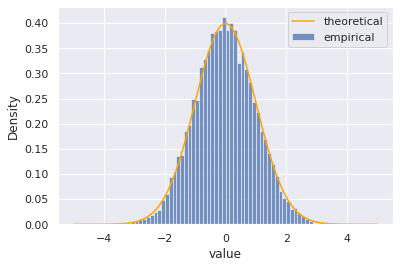
\includegraphics[width = 0.8\linewidth]{"./resources/norm_pair.png"}
	\caption{Демонстрация совпадения сгенерированного стандартного нормального
	 распределения с теоретическим при размере выборки $ n = 10000 $.}
    \label{fig:norm_pair}
\end{figure}

\anonsubsection{Критерий Фишера и t-критерий Стьюдента}
Проверим равенство дисперсий и матожиданий пары случайных величин построенных с
 помощью такого датчика. Для этого воспользуемся критерием Фишера и t-критерием
 Стьюдента.
\begin{definition}
	Случайная величина $ \zeta $ имеет $ F $-распределение(Фишера-Снедекора) с 
	 $k_1$ и $k_2$
	 степенями свободы(обозначается $ \zeta \sim F_{k_1,k_2}$), если
	$$
	 \zeta = \left. \left( \dfrac{1}{k_1} \xi \right) \right/ \left( \dfrac{1}{k_2}
	  \eta \right),
	$$
	где $ \xi \sim \chi_{k_1}^2, \ \eta \sim \chi_{k_2}^2 $, $ \xi $ и $ \eta $
	 независимы.
\end{definition}

\begin{definition}
	Пусть случайные величины $ Z $ и $ R_k^2 $ независимы и распределены согласно
	 законам $ \mathcal{N}(0,1) $ и $ \chi_k^2 $ соответственно. Тогда распределение
	 случайной величины $ T_k  = Z / \sqrt{R_k^2 / k} $ называют
	 распределением Стьюдента с k степенями свободы или t-распределением
	 (кратко $ T_k \sim t_k $).
\end{definition}

Критерий Фишера по сути может быть сформулирован следующим образом.
Если гипотеза $ H': \sigma_1 = \sigma_2, \ \mu_1 $ и $ \mu_2 $ --- любые 
 верна, то статистика $ S_1^2 / S_2^2 $ распределена по закону
 $ F_{n-1,m-1} $. Здесь
$$
S_1^2 = \frac{1}{n - 1} \sum_{i = 1}^{n}(X_i - \overline{X})^2, \quad
S_2^2 = \frac{1}{m - 1} \sum_{i = 1}^{m}(Y_i - \overline{Y})^2
$$
--- несмещенные оценки для дисперсий $ \sigma_1^2 $ и $ \sigma_2^2 $.
Это утверждение опирается на определение распределения Фишера и следующую теорему.
\begin{theorem}\footnote{Доказательство этой теоремы можно найти в
	\cite{lagutin_stat} на стр. 149.}
	Для нормальной выборки $ X_i \sim \mathcal{N}(\theta_1, \theta_2^2) $ Выборочное
	 среднее $ \overline{X} = \frac{1}{n}\sum X_i $ и выборочная дисперсия
	 $ S^2 = \frac{1}{n} \sum (X_i - \overline{X})^2 $ независимы, причем
	 $ n S^2 / \theta_2^2 \sim \chi_{n-1}^2 $, а $\sqrt{n - 1}
	 (\overline{X} - \theta_1) / S \sim t_{n-1} $.
\end{theorem}
В силу этой теоремы $ (n-1) S_1^2 / \sigma_1^2 \sim \chi_{n-1}^2,
 \ (m - 1) S_2^2 / \sigma_2^2 \sim \chi_{m-1}^2 $, и следовательно
 формулировка критерия Фишера верна. Отметим, что критерий Фишера имеет
 двустороннюю критическую область, поэтому сравнение статистики для отвержения
 или принятия гипотезы в этом случае нужно проводить и с $ \dfrac{\alpha}{2} $
 - квантилью и с $ 1 - \dfrac{\alpha}{2} $ - квантилью распределения
 Фишера-Снедекора. \medskip\\
Проверим теперь равенство математических ожиданий с помощью критерия Стьюдента.
 Обозначим неизвестную общую дисперсию через $ \sigma^2 $. Так как распределение
 хи-квадрат является частным случаем гамма-распределения $(\chi_k^2 
 \sim \Gamma(k/2, 1/2)) $, получаем
$$
 \sigma^{-2} \left[(n - 1) S_1^2 + (m - 1) S_2^2 \right] \sim \chi_{n + m - 2}^2.
$$
Поскольку математическое ожидание закона $ \chi_{n + m - 2}^2 $ равно $ n + m - 2 $,
 статистика $ S_{tot}^2 = \left[(n - 1) S_1^2 + (m - 1) S_2^2 \right] / (n + m -2) $
 несмещенно оценивает $ \sigma^2 $ по объединенной выборке.

При справедливости гипотезы $ H^{''}: \mu_1 = \mu_2 $ ввиду независимости выборок
 имеем: $\overline{X} - \overline{Y} \sim \mathcal{N}(0, (1/n + 1/m)\sigma^2) $.
 Отсюда согласно определению закона Стьюдента:
$$
T = \left( \overline{X} - \overline{Y} \right) \left/ \left( S_{tot}
 \sqrt{\dfrac{1}{n} + \dfrac{1}{m}} \right) \right. = \left. \sqrt{\dfrac{nm}{n + m}} \left(\overline{X}
 - \overline{Y} \right) \right/ S_{tot} \sim t_{n + m - 2}.
$$
Это приводит к критерию Стьдента, позволяющему проверить гипотезу $ H^{''} $.
 Отметим также, что данный критерий, как и критерий Фишера имеет двустороннюю критическую
 область.

\begin{thebibliography}{0}
	\addcontentsline{toc}{section}{Список литературы}
	\bibitem{lagutin_stat} Лагутин~М.\,Б.
	\emph{Наглядная метематическая статистика}, Бином. М.: 2009.
	
	\bibitem{model_randoms} Кропачёва~Н.\,Ю., Тихомиров~А.\,С.
	\emph{Моделирование случайных величин}, НовГУ им. Ярослава
     Мудрого. Великий Новгород: 2004.

	\bibitem{shir_prob} Ширяев~А.\,Н.
	\emph{Вероятность}, МЦНМО. М.: 2007.
\end{thebibliography}
\end{document}